\documentclass{beamer}
%\beamerdefaultoverlayspecification{<+->}

\usetheme{metropolis}
\usepackage{graphicx}
\usepackage{amsmath}
\usepackage{mathtools}
\usepackage{minted}

\title{Neural Networks for Image Classification}
\date{\today}
\author{Catalina Vajiac}
\institute{Saint Mary's College} 
\setminted{fontsize=\small, baselinestretch=1}
\begin{document}
  \maketitle

  \section{Introduction}
  \begin{frame}{Overview}
    \begin{itemize}
      \item Motivation for neural networks
      \item What is a neural network?
      \begin{itemize}
        \item fully-connected
        \item deep
      \end{itemize}
      \item Gradient Descent
      \begin{itemize}
        \item Softmax classifier
        \item single-layer neural network
        \item arbitrary-layer neural network
      \end{itemize}
      \item Demonstration
        \begin{itemize}
          \item comparison of networks on MNIST
        \end{itemize}
    \end{itemize}
  \end{frame}

  \section{Motivation}
  \begin{frame}{What's the Point?}
    \begin{figure}[ht!] \centering
      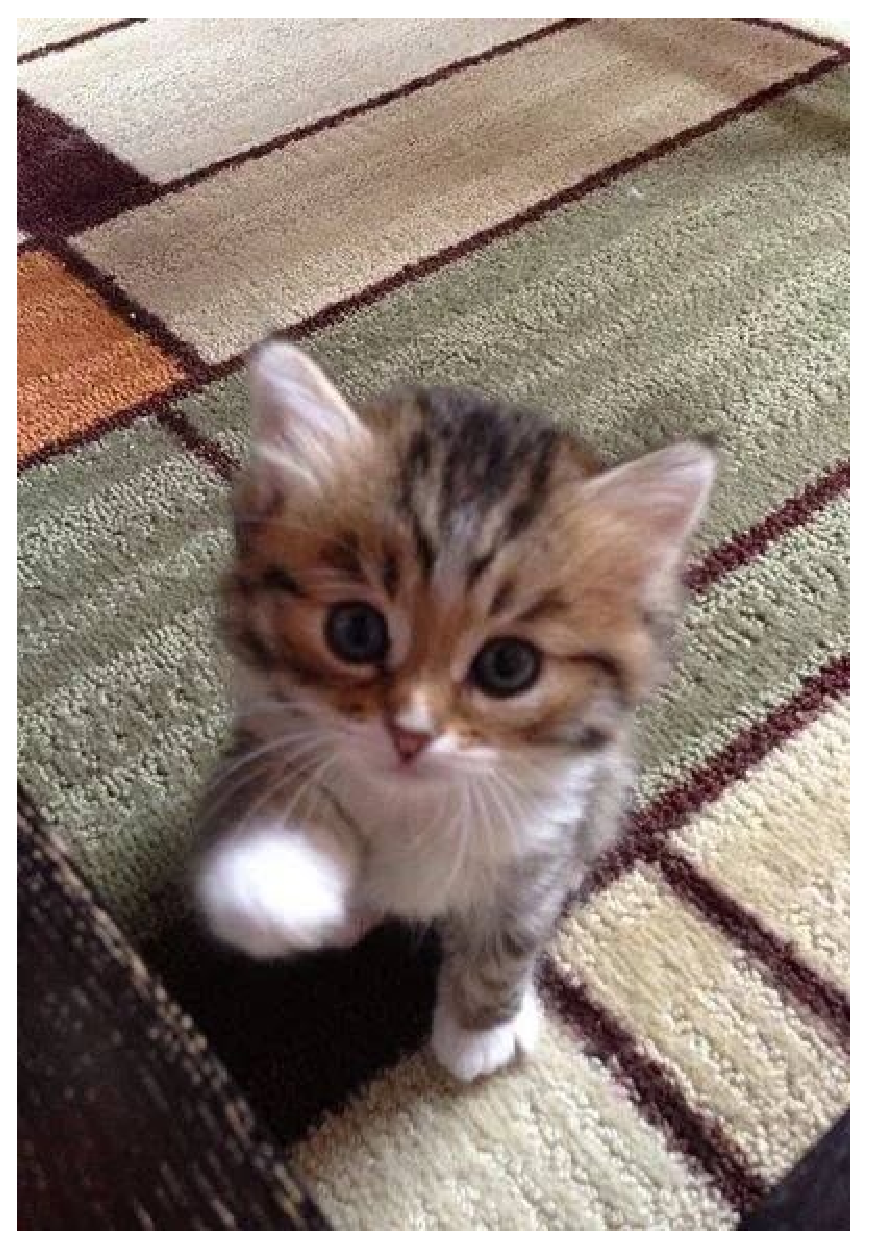
\includegraphics[height=2.5in]{../figures/kitty.eps}
    \end{figure}
    What's in this image?
  \end{frame}

  \begin{frame}{Image Variation}
    \begin{figure}[ht!] \centering
      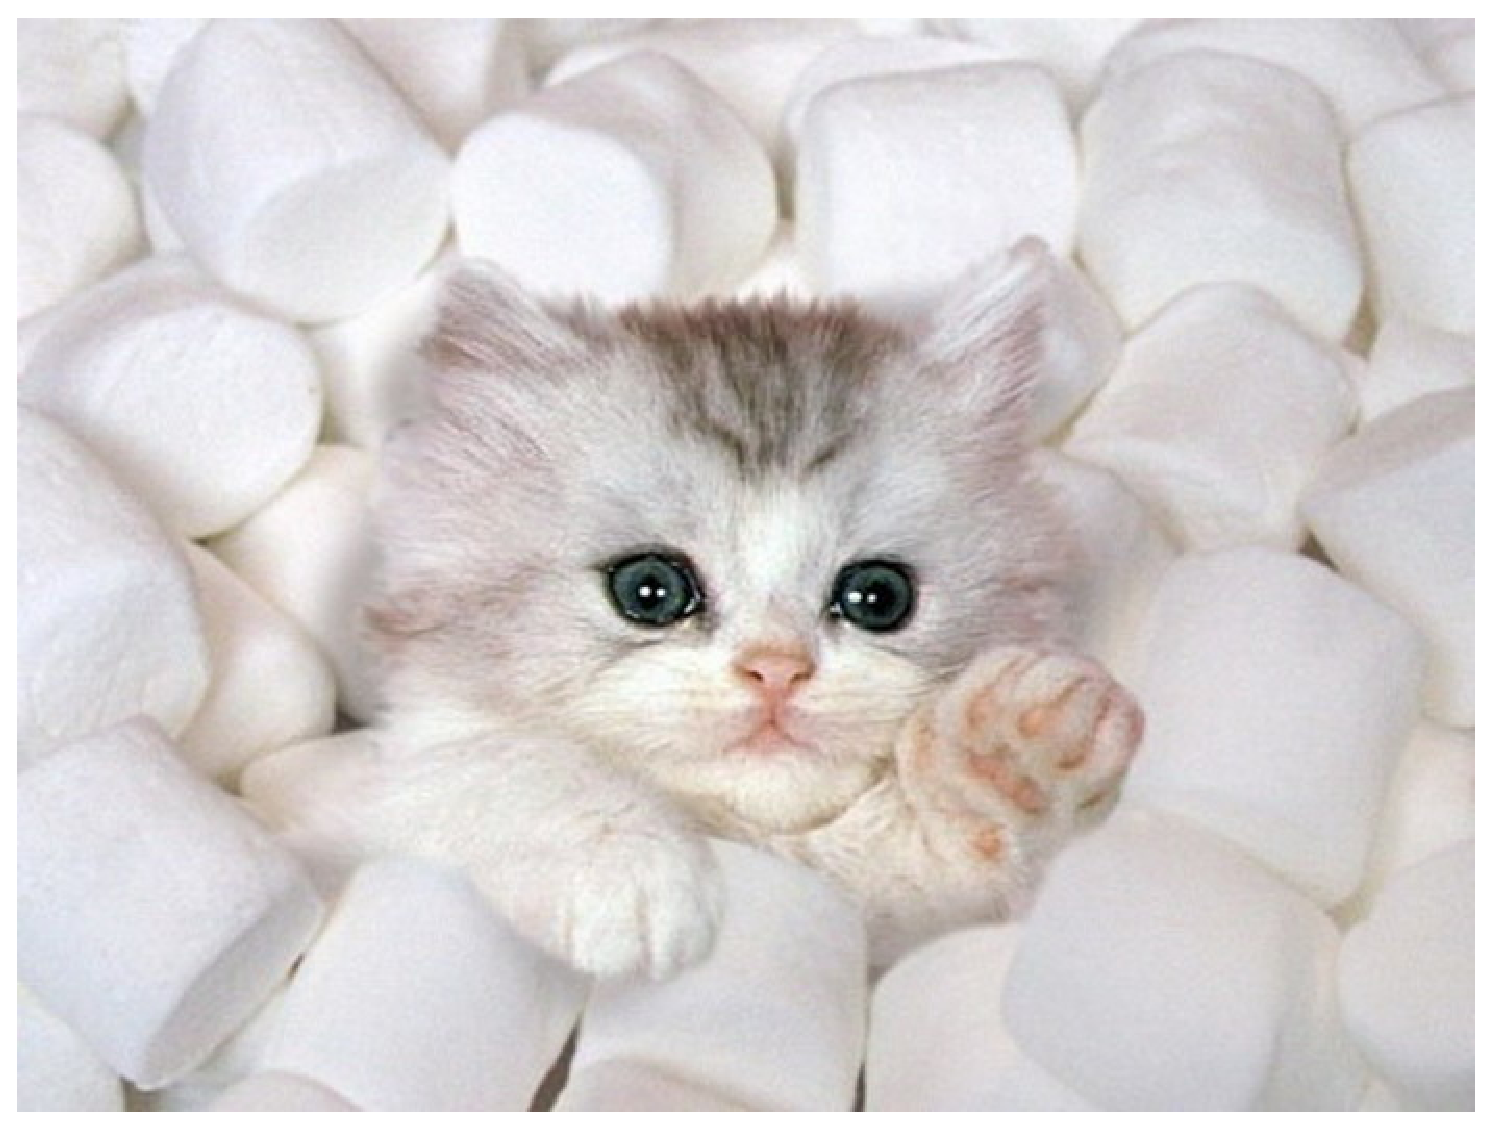
\includegraphics[height=1.2in]{../figures/kitty_occlusion.eps}
      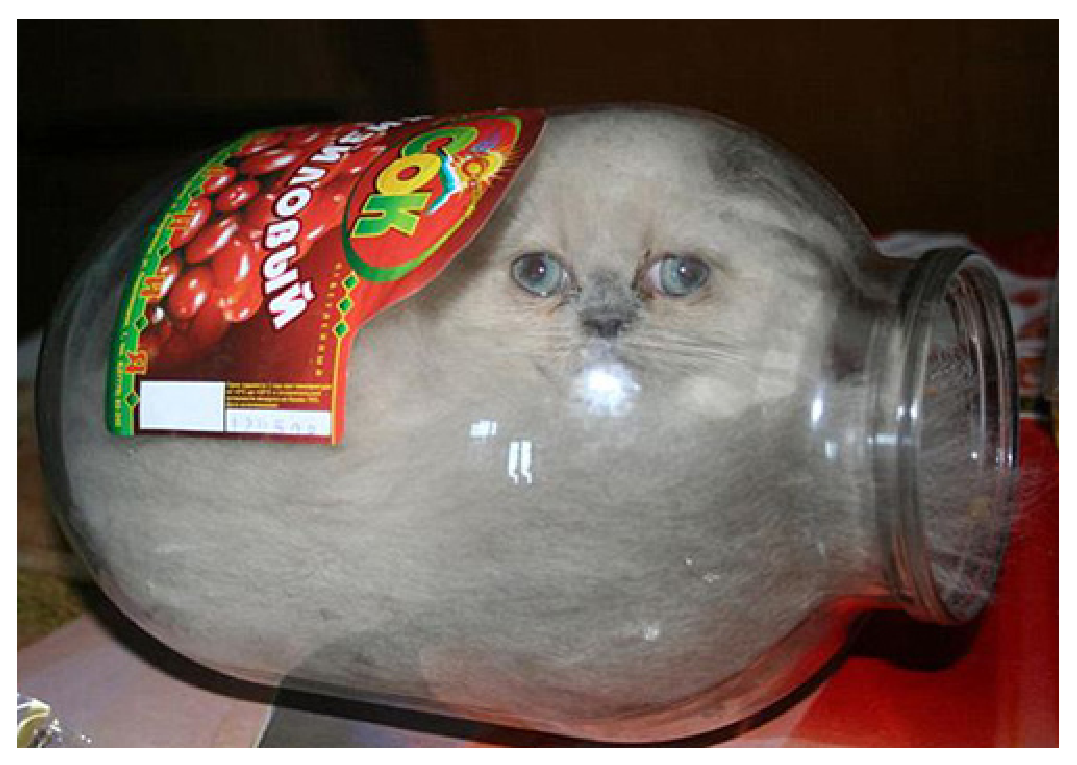
\includegraphics[height=1.2in]{../figures/cat_deformed.eps}
      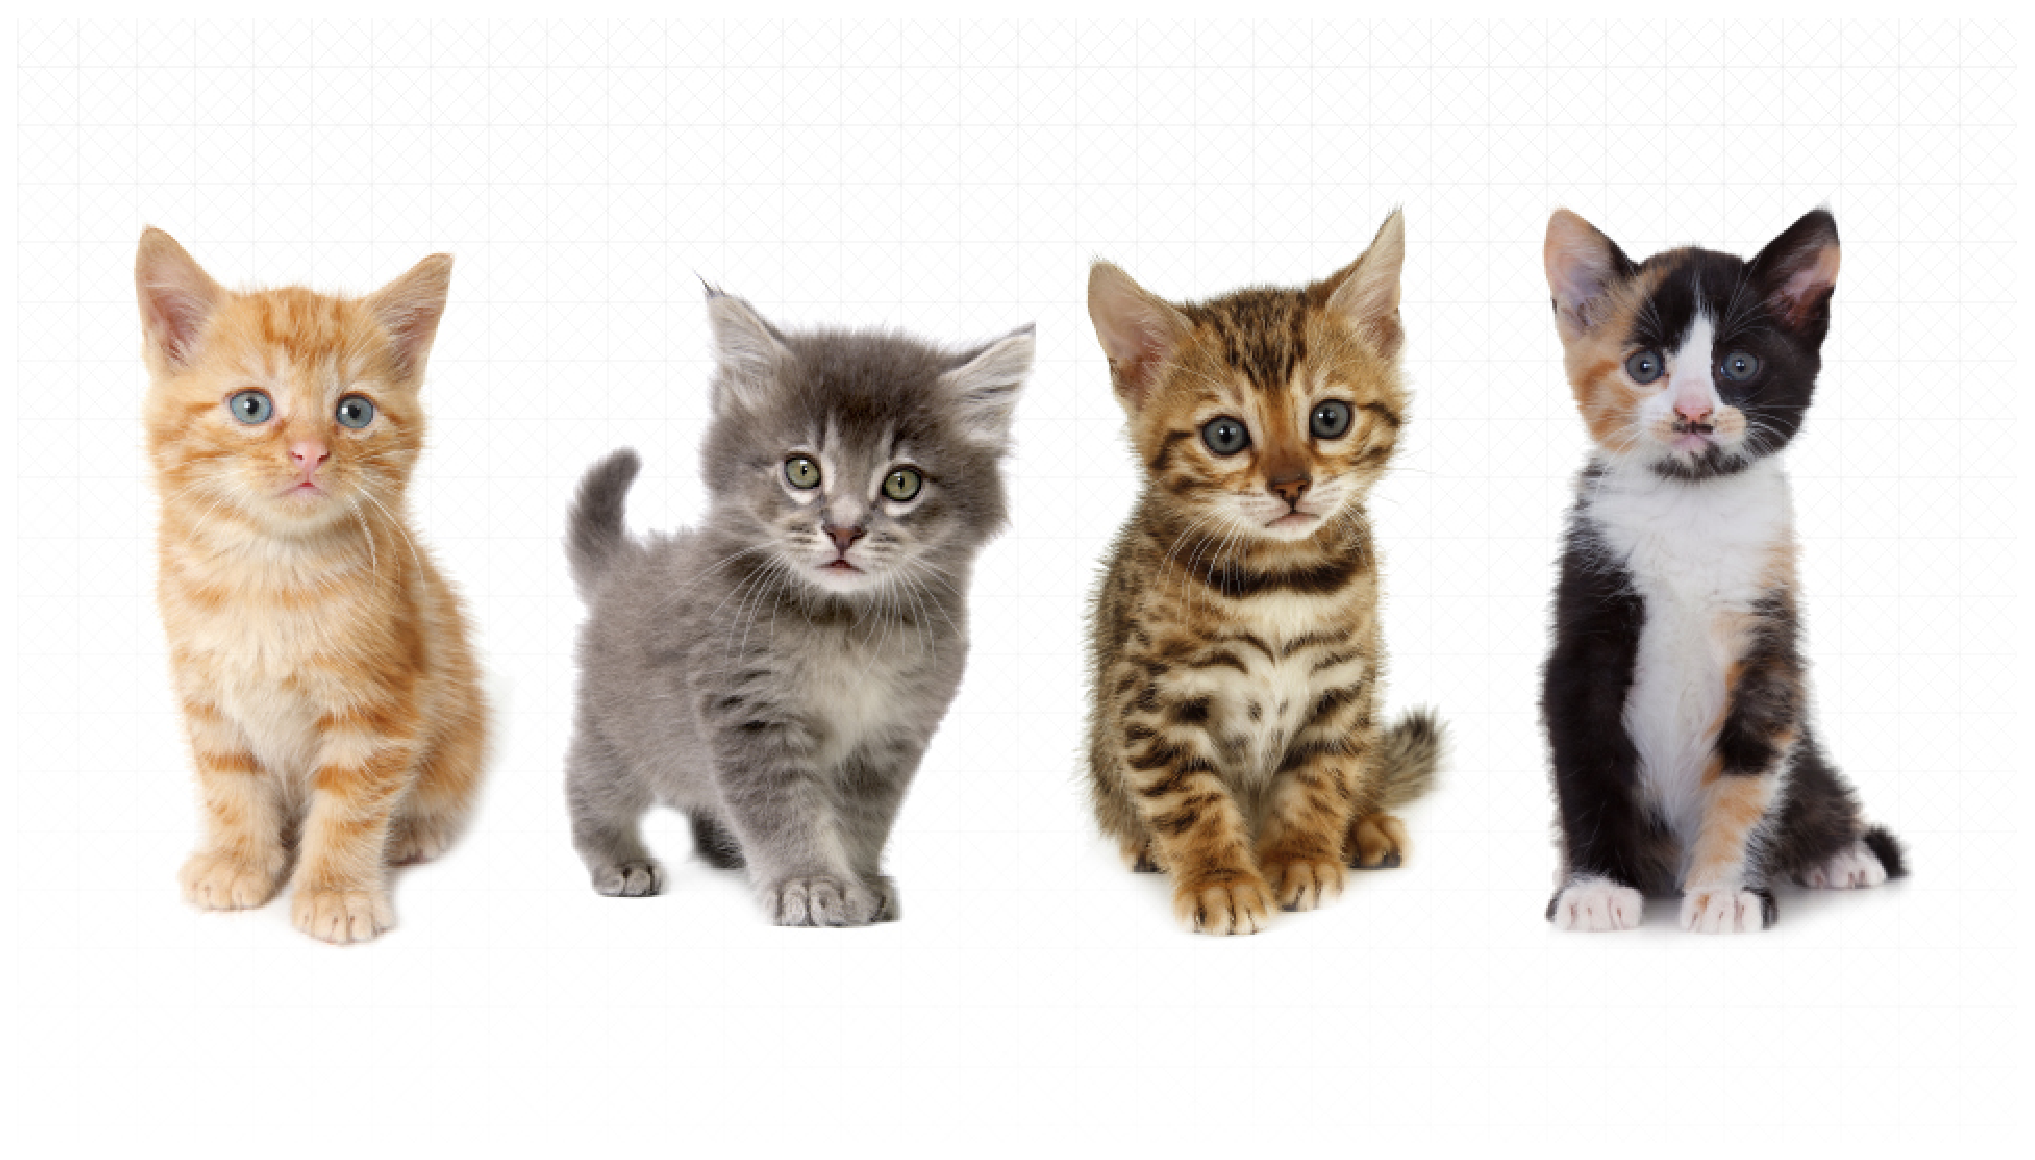
\includegraphics[height=2in]{../figures/kitty_intra_class_variation.eps}
    \end{figure}

  \end{frame}

  \section{Neural Networks}
  \begin{frame}{What is a Neural Network?}
    \begin{itemize}
      \item collection of units (neurons) that transmit signals to one another
      \item each unit processes signal, propagates forward
      \item allows computer to learn from observational data
    \end{itemize}
    \begin{center}
      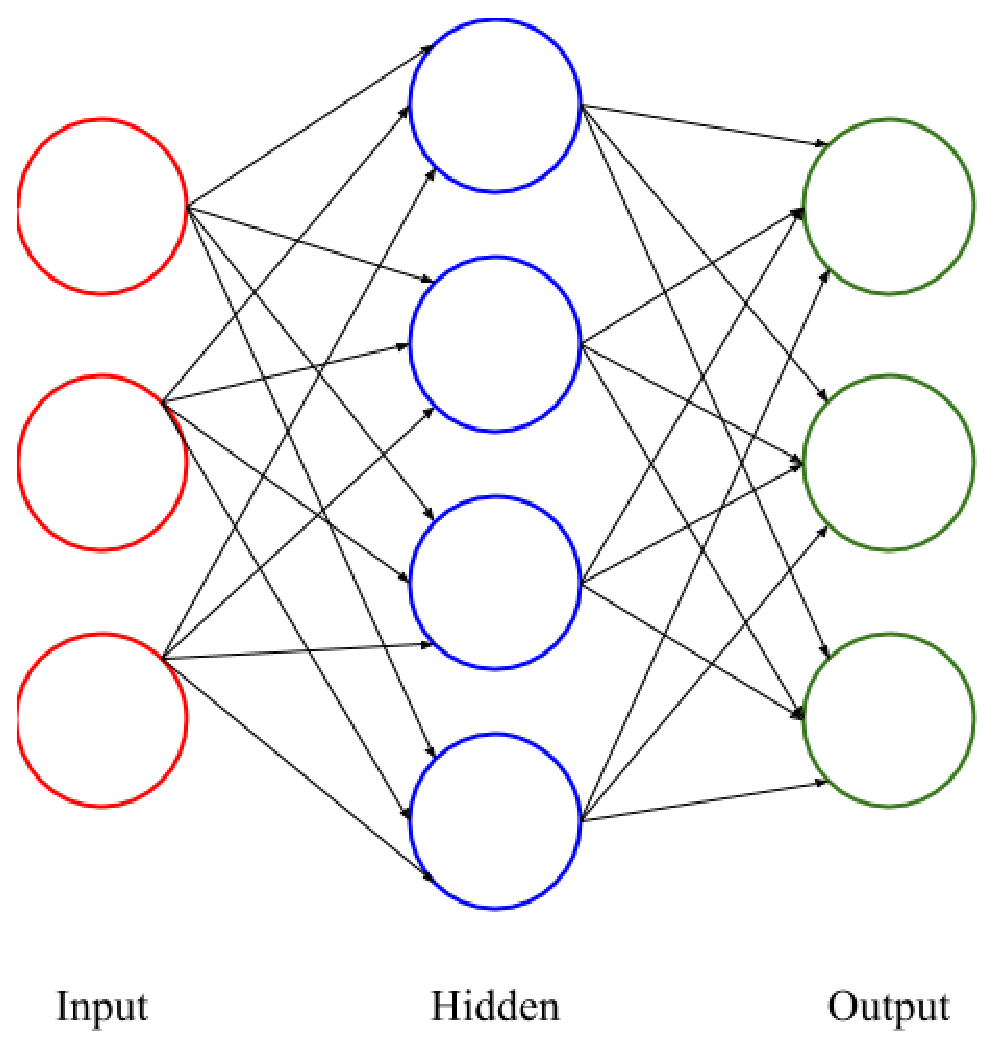
\includegraphics[height=2in]{../figures/neural_network.eps}
    \end{center}
  \end{frame}

  \begin{frame}{Deep Neural Network}
    \begin{figure}[ht!]
      \centering
      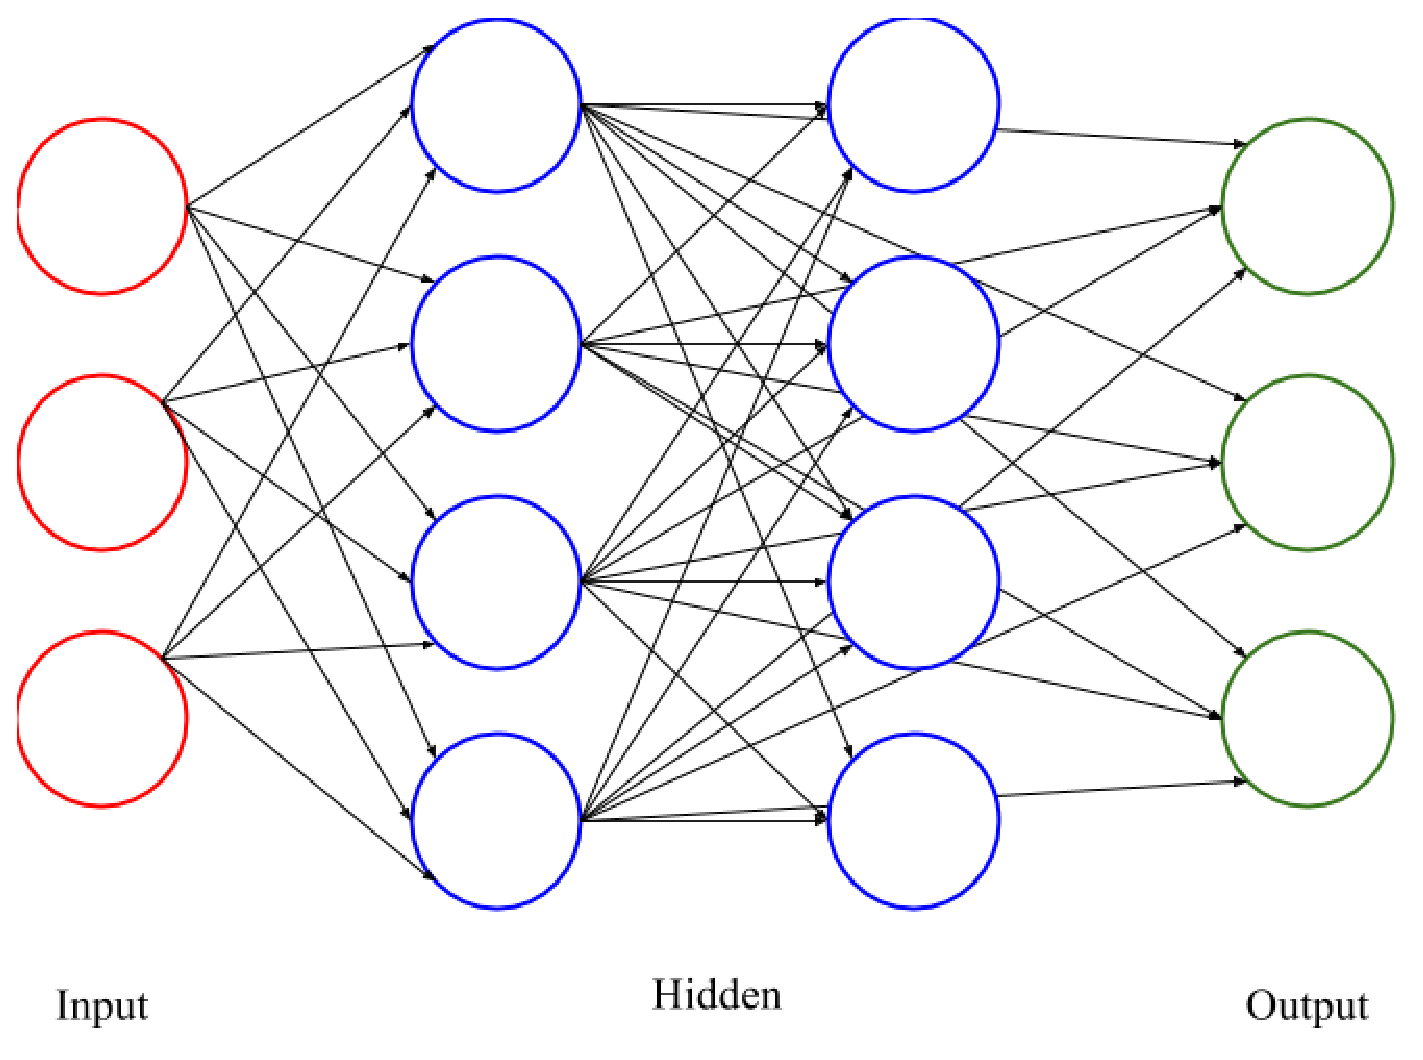
\includegraphics[height=2in]{../figures/deep_nn.eps}
      \caption{Visualization of a deep neural network}
      \label{fig:dnn}
    \end{figure}
  \end{frame}

  \begin{frame}{Datasets: MNIST}
    \begin{itemize}
      \item handwritten digit recognition
      \item $28 \times 28$ pixel, greyscale
      \item 60,000 training images, 10,000 testing images
    \end{itemize}
    \begin{center}
      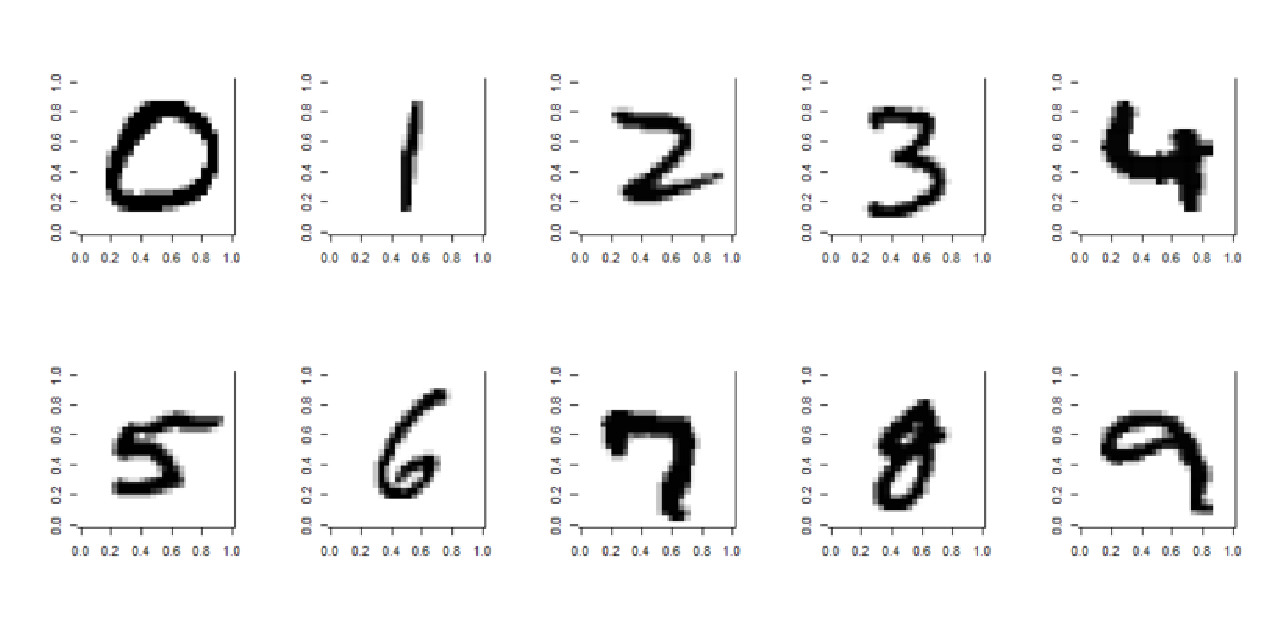
\includegraphics[height=2in]{../figures/mnist.eps}
    \end{center}
  \end{frame}

  \begin{frame}{Linear Classification}
    Essentially a 0-layer* neural network\\
    Linear classification has two important parts:
    \begin{itemize}
      \item prediction function: maps data to class scores
      \item loss function: compares predicted scores with actual labels
    \end{itemize}
  \end{frame}

  \begin{frame}{Prediction Function}
    How likely is it that each training example is part of any class?
    $$ P = XW + b $$
    \begin{itemize}
      \item $X$: training data
      \item $W$: weights
      \item $b$: bias vector
    \end{itemize}
  \end{frame}

  \begin{frame}{Loss Function}
    Evaluates $P$ based on actual data labels
    $$ L = \sum_{i=1}^m L_i(P_i, y_i). $$
    \begin{itemize}
      \item $y$: labels for training data
      \item $L_i$: loss for one training example
      %\item $L$: overall loss over entire training dataset
    \end{itemize}
    $$ L_i(P) = -\frac{1}{m} \left[ P_{iy_i} - \log\left( \sum_{j=1}^k \exp
    P_{ij} \right)\right] $$ for all $i$ where $1 \leq i \leq m$.
  \end{frame}

  \begin{frame}{Gradient Descent}
    Goal: find optimal $W$ and $b$ by minimizing $L$\\
    Steps of Gradient Descent:
    \begin{enumerate}
      \item forward propogation: \begin{itemize}
        \item calculate prediction function
      \end{itemize}
      \item back propogation: \begin{itemize}
        \item calculate $\nabla P$
        \item use $\nabla P$ to calculate gradients w.r.t. model parameters
      \end{itemize}
      \item update $W$ and $b$ accordingly
    \end{enumerate}
  \end{frame}

  \section{Softmax Classifier}

  \begin{frame}{Softmax Classifier: What can it do?}
    \begin{center}
      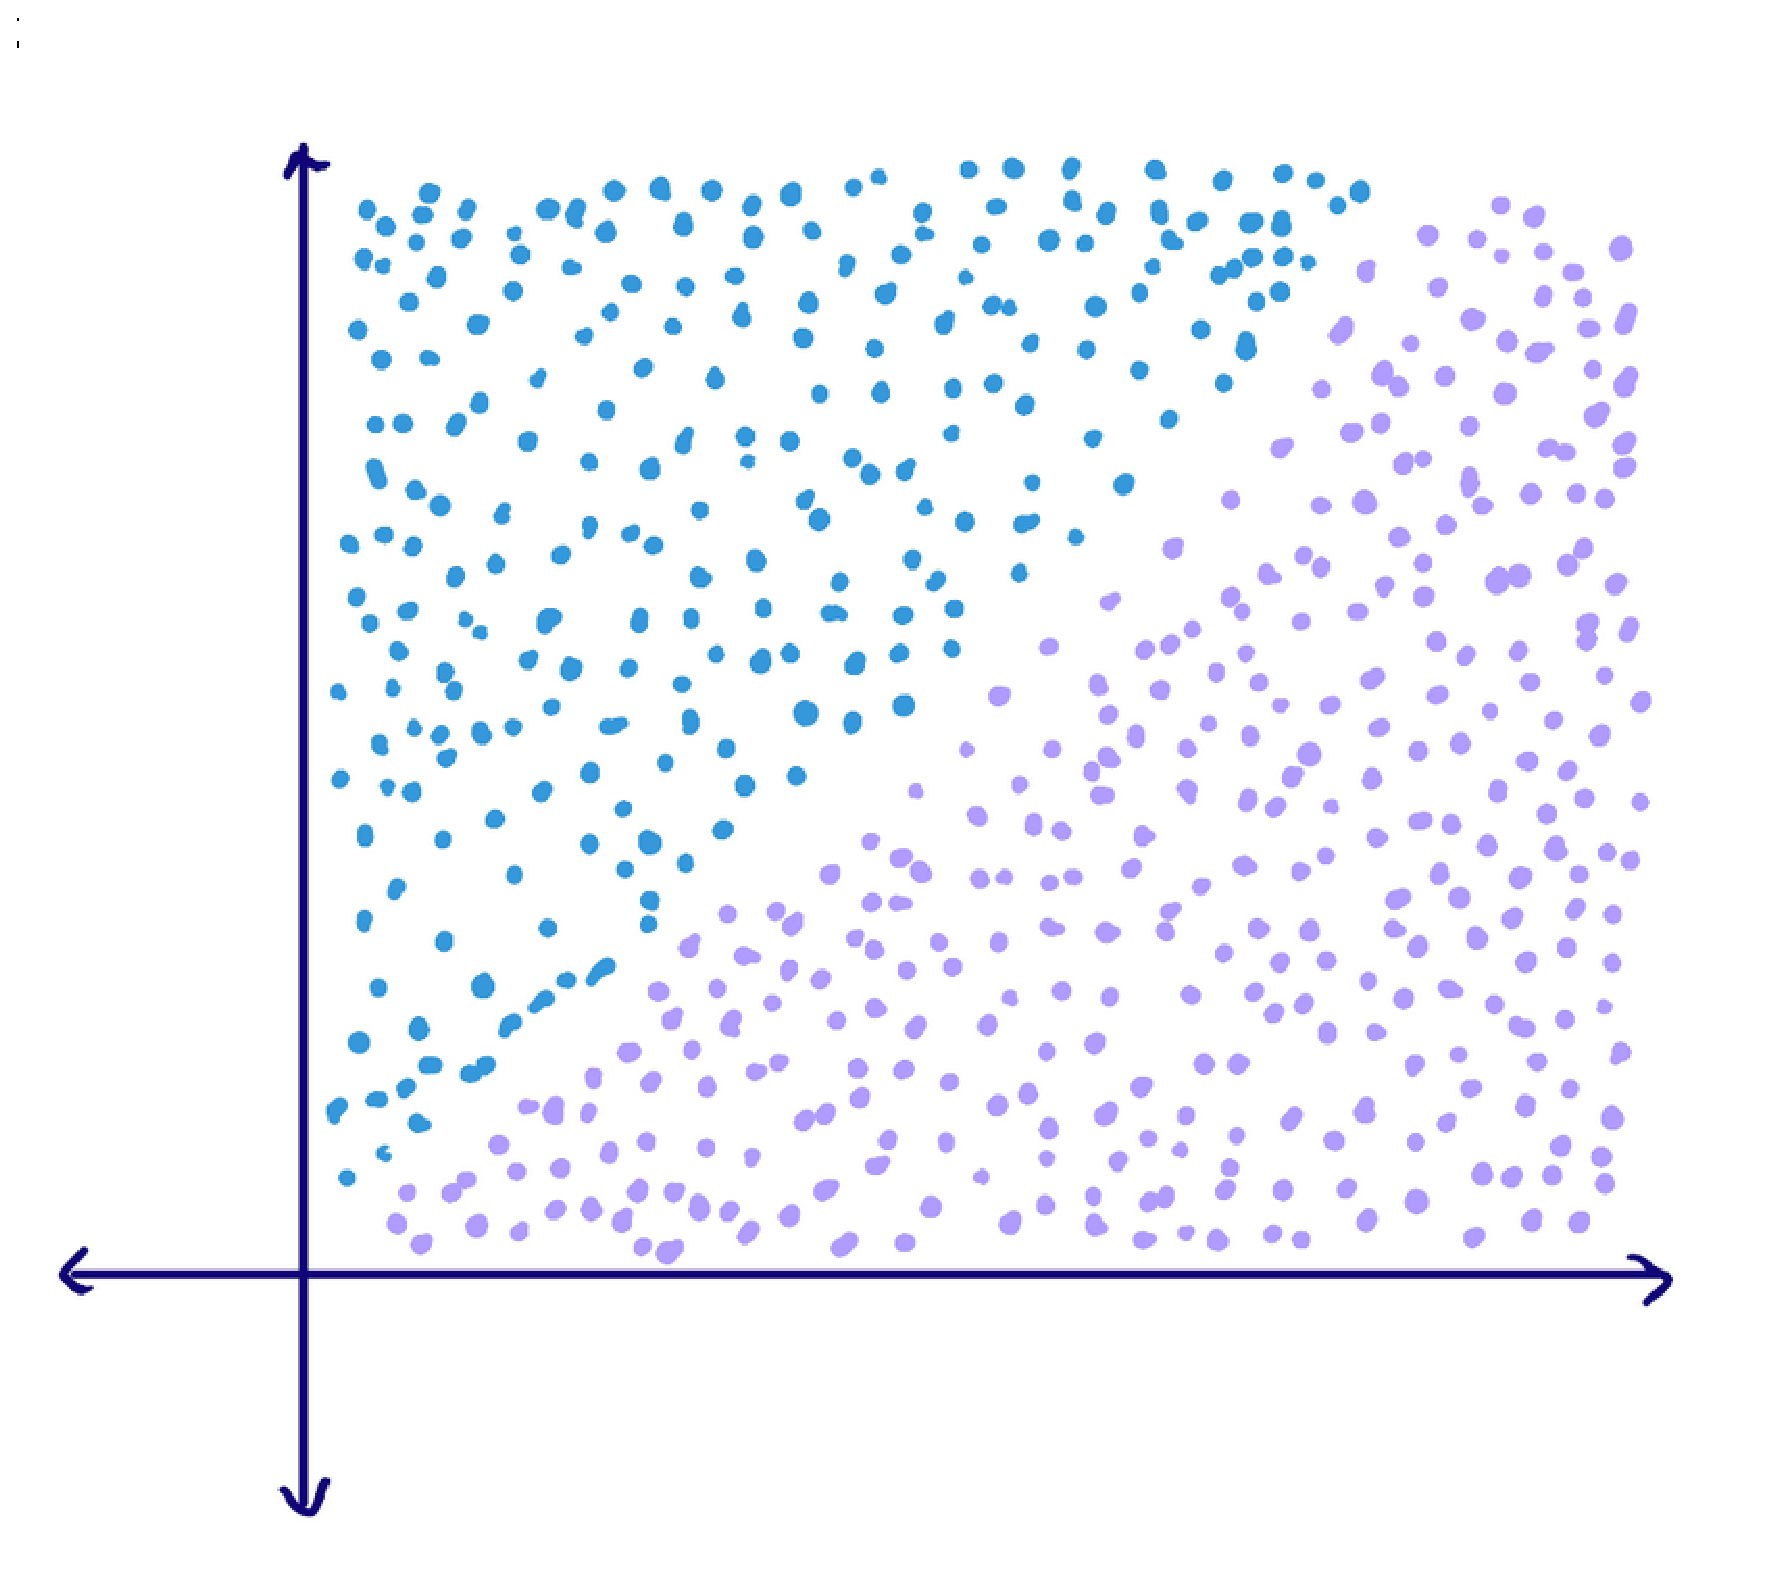
\includegraphics[width=3in]{../figures/linear.eps}
    \end{center}
  \end{frame}

  \begin{frame}{Softmax Classifier: What does it look like?}
    \begin{center}
      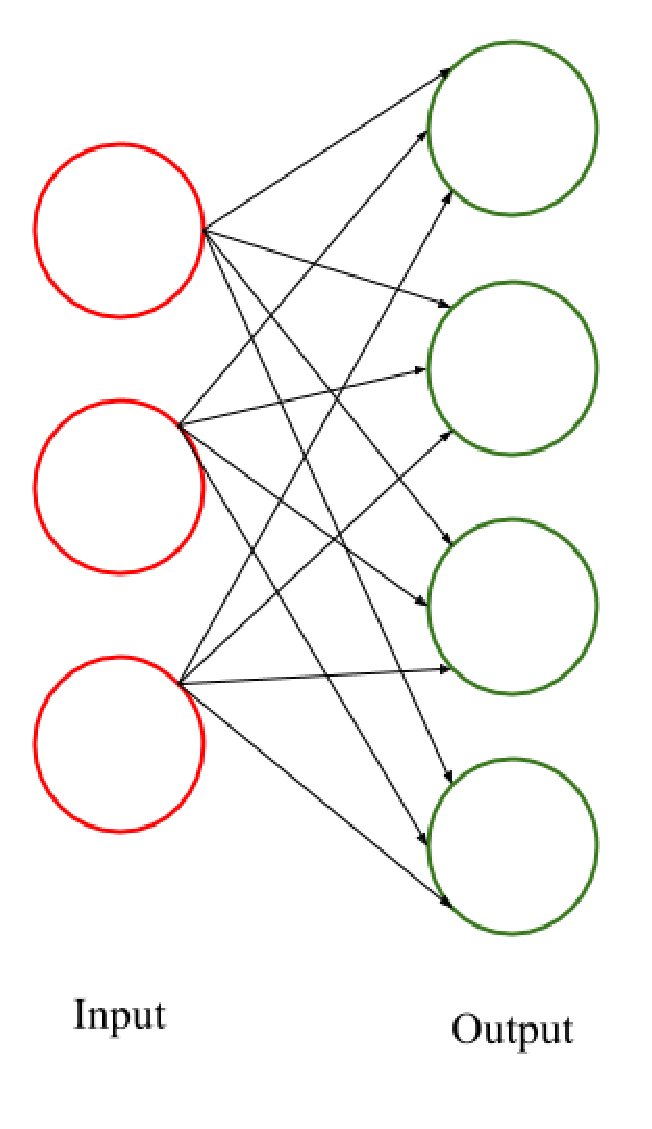
\includegraphics[width=1.5in]{../figures/linear_classifier.eps}
    \end{center}
  \end{frame}

  \begin{frame}{Softmax Classifier}
    Forward propagation:
    $$ P = XW + b. $$
    Back propagation:
    \begin{itemize}
      \item calculate $\nabla P$
      \item calculate $\nabla W$, $\nabla b$
    \end{itemize}
    Gradient update:
    $$ W = W - \eta \nabla W. $$
    $$ b = b - \eta \nabla b. $$
  \end{frame}

  \begin{frame}{Softmax Classifier: Deriving $\nabla W$}
    Recall:
    $$ \nabla P = -\frac{1}{m} \left[ Y -
    \frac{\exp{P_{uv}}}{\sum_{i=1}^m\exp{P_{ij}}} \right], $$
    $$ \nabla W = X^T \nabla P, $$
    $$ \nabla b = \sum_{j=0}^k P_j. $$
  \end{frame}

  \begin{frame}{Softmax Classifier: Gradient Descent Update}
    Update $W$ and $b$:
    \begin{center}
      $$ W = W - \eta \nabla W, $$
      and
      $$ b = b - \eta \nabla b, $$
      where $\eta$ is the learning rate.
    \end{center}
  \end{frame}

  \begin{frame}{Single Layer: Deriving $\nabla X$}
    \begin{align*}
      \frac{\partial L}{\partial X_{uv}} 
      =\sum_{i=1}^m \frac{\partial L_i}{X_{uv}}
      &= \sum_{i=1}^m \sum_{j=1}^k \frac{\partial L_i}{\partial P_{ij}}
          \frac{\partial P_{ij}}{\partial X_{uv}}\\
      &= \sum_{i=1}^m \sum_{j=1}^k \frac{\partial L_i}{\partial P_{ij}}
          1(i == u) W_{vj}\\
      &= \sum_{j=1}^k \sum_{i=1}^m \frac{\partial L_i}{\partial P_{ij}}
          1(i == u) W_{vj}\\
      &= \sum_{j=1}^k \frac{\partial L_u}{\partial P_{uj}} W_{vj}\\
      &= \sum_{j=1}^k \nabla P_{uj} W_{vj}
       = \left( \nabla P W^T \right) _{uv}.
    \end{align*}
    $$ \nabla X = \nabla P W^T. $$
  \end{frame}

  \begin{frame}{Single Layer: What can it do?}
    \begin{center}
      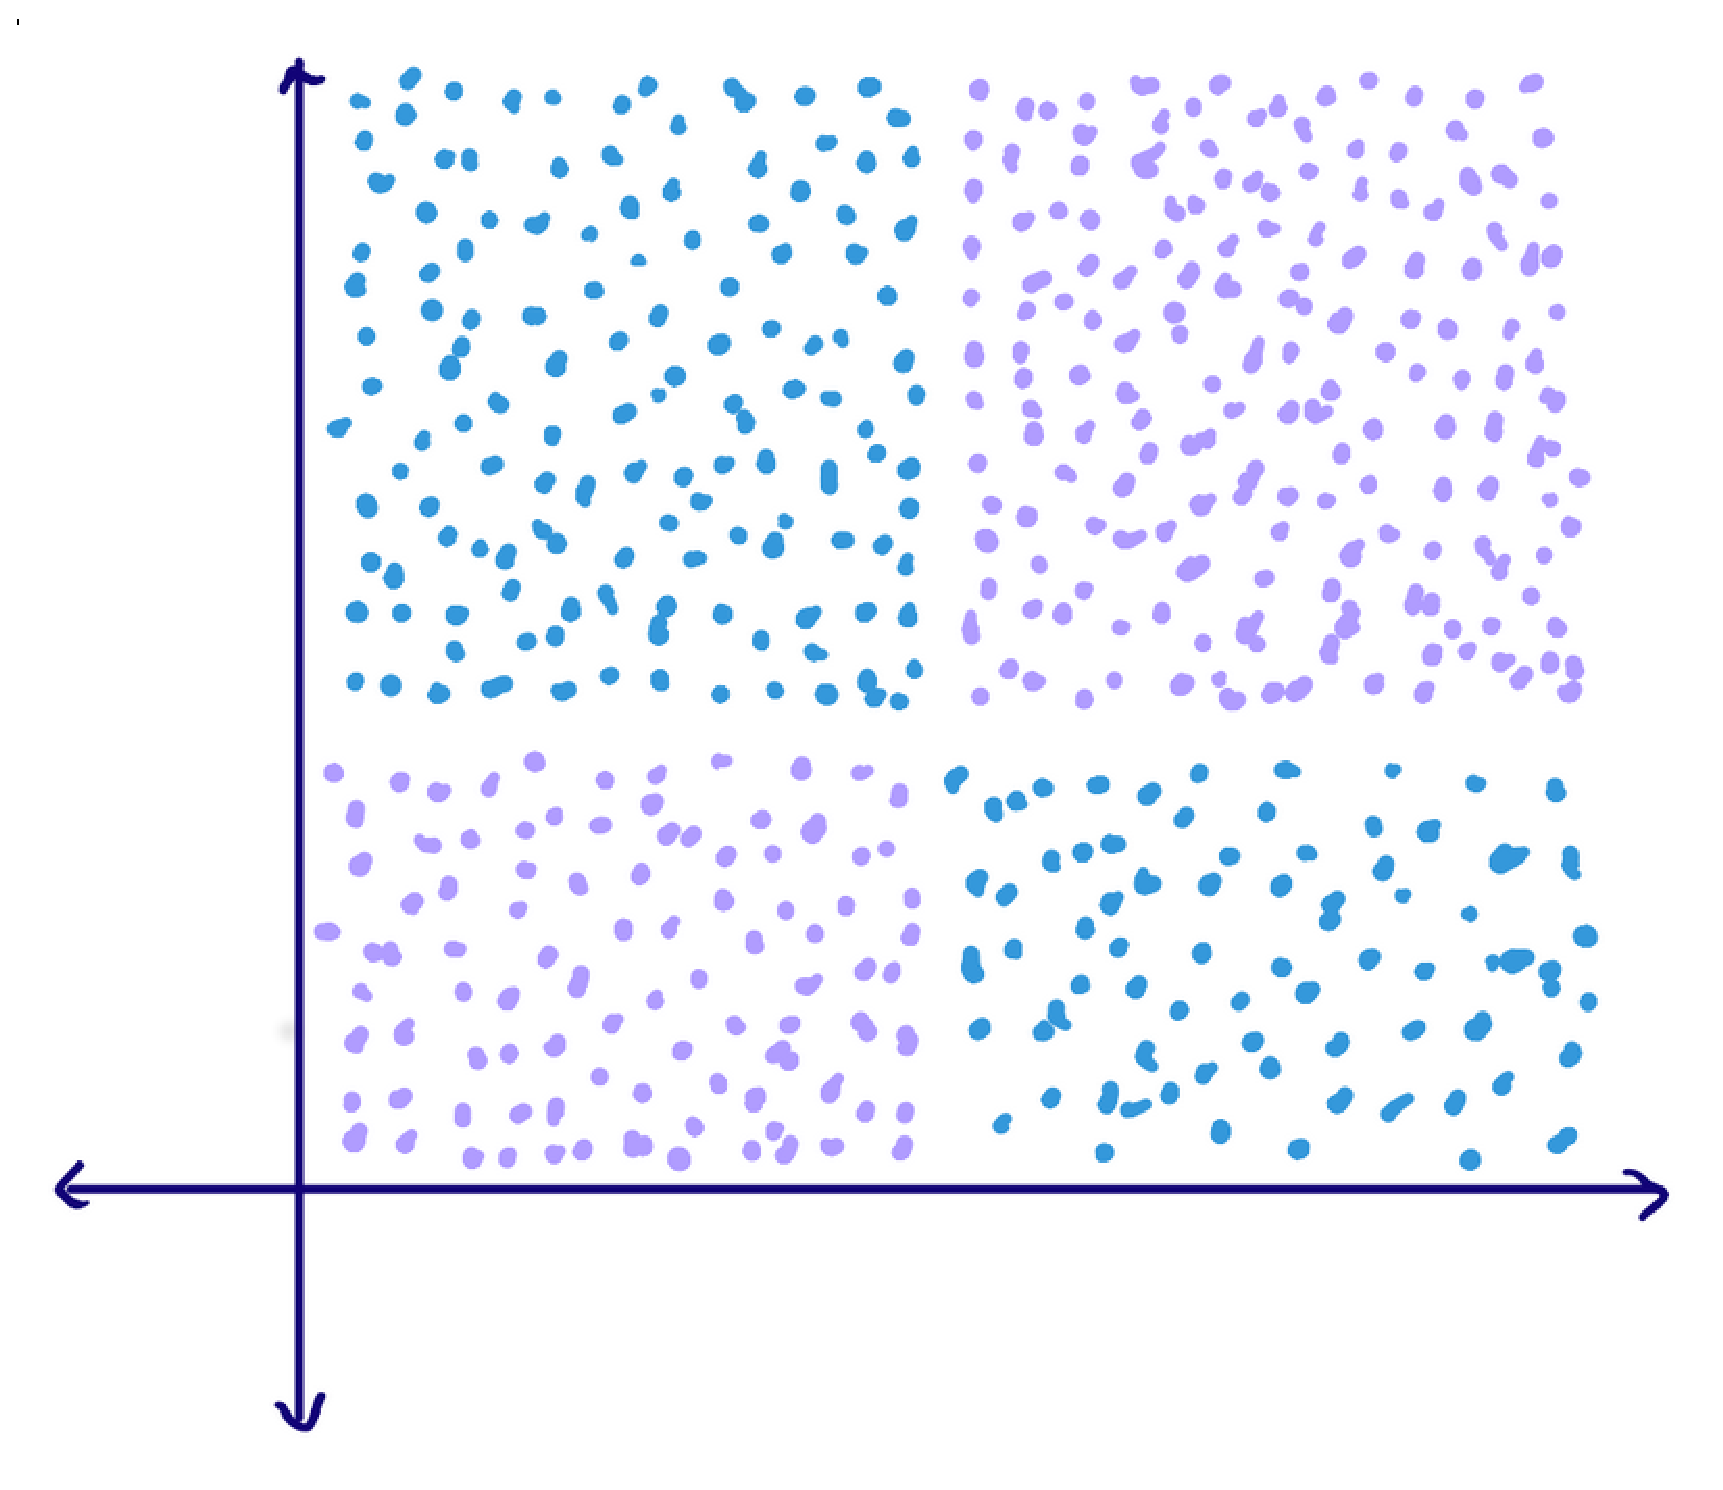
\includegraphics[width=3in]{../figures/onelayer.eps}
    \end{center}
  \end{frame}

  \begin{frame}{Single Layer: What does it look like?}
    \begin{center}
      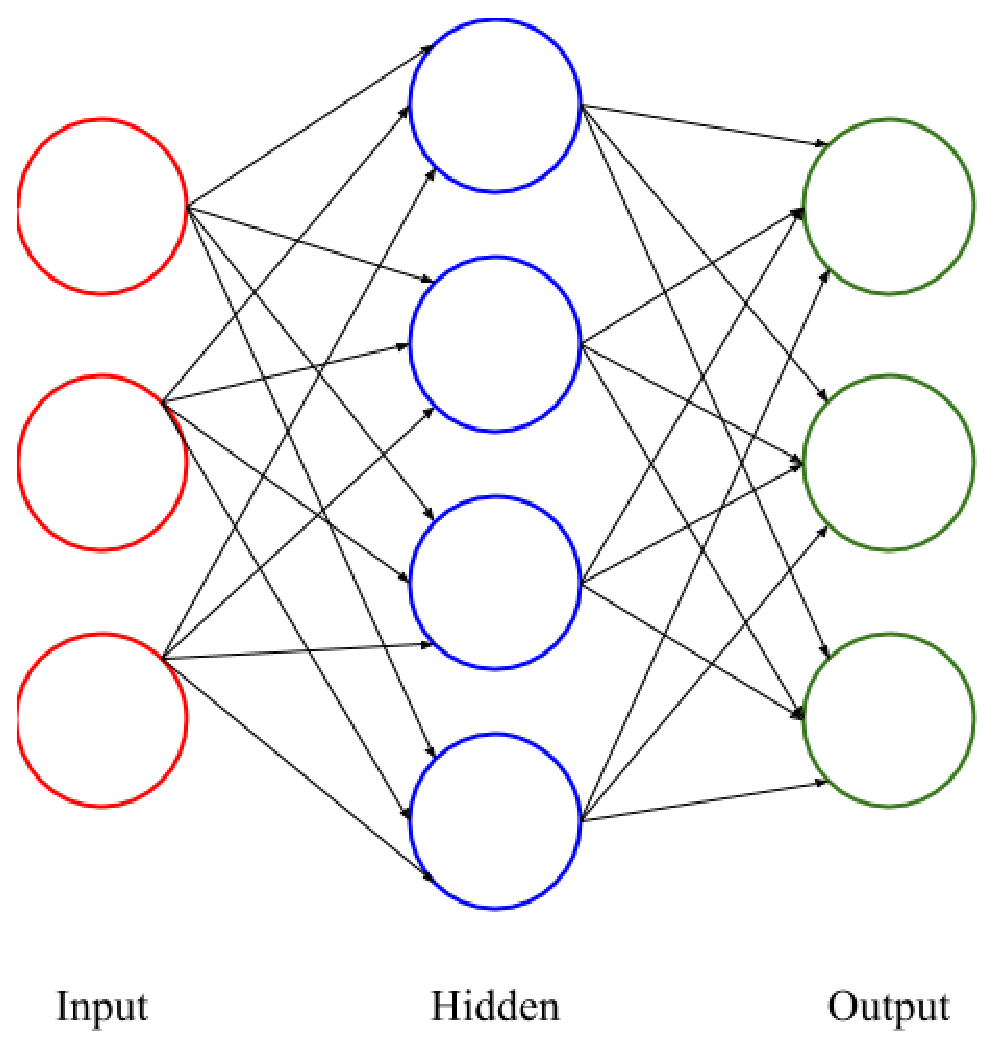
\includegraphics[width=2.5in]{../figures/neural_network.eps}
    \end{center}
  \end{frame}

  \section{Single Layer Neural Network}
  \begin{frame}{Single Layer}
    Steps:
    \begin{enumerate}
      \item Forward propogation:
      \begin{itemize}
        \item $ A = XW^{(1)} + b^{(1)} $
        \item $ Z = \phi(A) $
        \item $ P = ZW^{(2)} + b^{(2)} $
      \end{itemize}

      \item Backward propogation:
      \begin{itemize}
        \item calculate $\nabla W^{(1)}, \nabla W^{(2)}, \nabla b^{(1)},
              \nabla b^{(1)}, \nabla Z$
      \end{itemize}

      \item Update weights:
      \begin{itemize}
        \item e.g. $W^{(1)} = W^{(1)} - \eta \nabla W^{(1)}$
      \end{itemize}
    \end{enumerate}
  \end{frame}

  \begin{frame}{Single Layer: ReLU function}
    $$ \phi(x) = relu(x) =
      \begin{cases}
        0 & x < 0\\
        x & x \geq 0
      \end{cases}.$$

  Note : $\phi(x)$ is not differentiable at $x = 0$.

  Use $1(x == 0)$ instead
  \end{frame}

  \begin{frame}{Single Layer: Deriving $\nabla W^{(2)}$, $\nabla
  b^{(2)}$, $\nabla W^{(1)}$, $\nabla b^{(1)}$}
    Note: $\nabla W^{(2)}$, $\nabla b^{(2)}$ are identical to $W, b$ in a Softmax Classifier, so
    $$ \nabla W^{(2)} = Z^T \nabla P, $$
    $$ \nabla b^{(2)} = \sum_{i=1}^m P_i. $$

    Similarly, $\nabla W^{(1)}$, $\nabla b^{(1)}$ will be
    $$ \nabla W^{(1)} = X^T \nabla A, $$
    $$ \nabla b^{(1)} = \sum_{i=1}^m A_i.$$
  \end{frame}

  \begin{frame}{Single Layer: Deriving $\nabla Z$}
    
    $\nabla Z$ is analagous to $\nabla X$ in the Softmax classifier, so

    $$ \nabla Z = \nabla P W^{(2)T}. $$
      
  \end{frame}

  \begin{frame}{Single Layer: Deriving $\nabla A$}
    \begin{align*}
      \frac{\partial L}{\partial A_{uv}}
      &= \sum_{i=1}^m \frac{\partial L_i}{\partial A_{uv}}\\
      &= \sum_{i=1}^m \frac{\partial L_i}{\partial Z_{uv}} \frac{\partial
         Z_{uv}}{\partial A_{uv}}\\
      &= \frac{\partial L_u}{Z_{uv}} 1(A_{uv} > 0)\\
      &= \nabla Z_{uv} 1(A_{uv} > 0).
    \end{align*}

    So we have
    $$ \nabla A = \nabla Z \bullet 1(A > 0), $$

    where $\bullet$ indicates element-wise multiplication.
  \end{frame}

  \begin{frame}{Single Layer: Update}
    Parameter update is similar:
      $$ W^{(1)} = W^{(1)} - \eta \nabla W^{(1)}. $$
      $$ b^{(1)} = b^{(1)} - \eta \nabla b^{(1)}. $$
      $$ W^{(2)} = W^{(2)} - \eta \nabla W^{(2)}. $$
      $$ W^{(2)} = W^{(2)} - \eta \nabla W^{(2)}. $$
  \end{frame}

  \section{Arbitrary Layer Neural Network}
  \begin{frame}{Arbitrary Layer: What can it do?}
    \begin{center}
      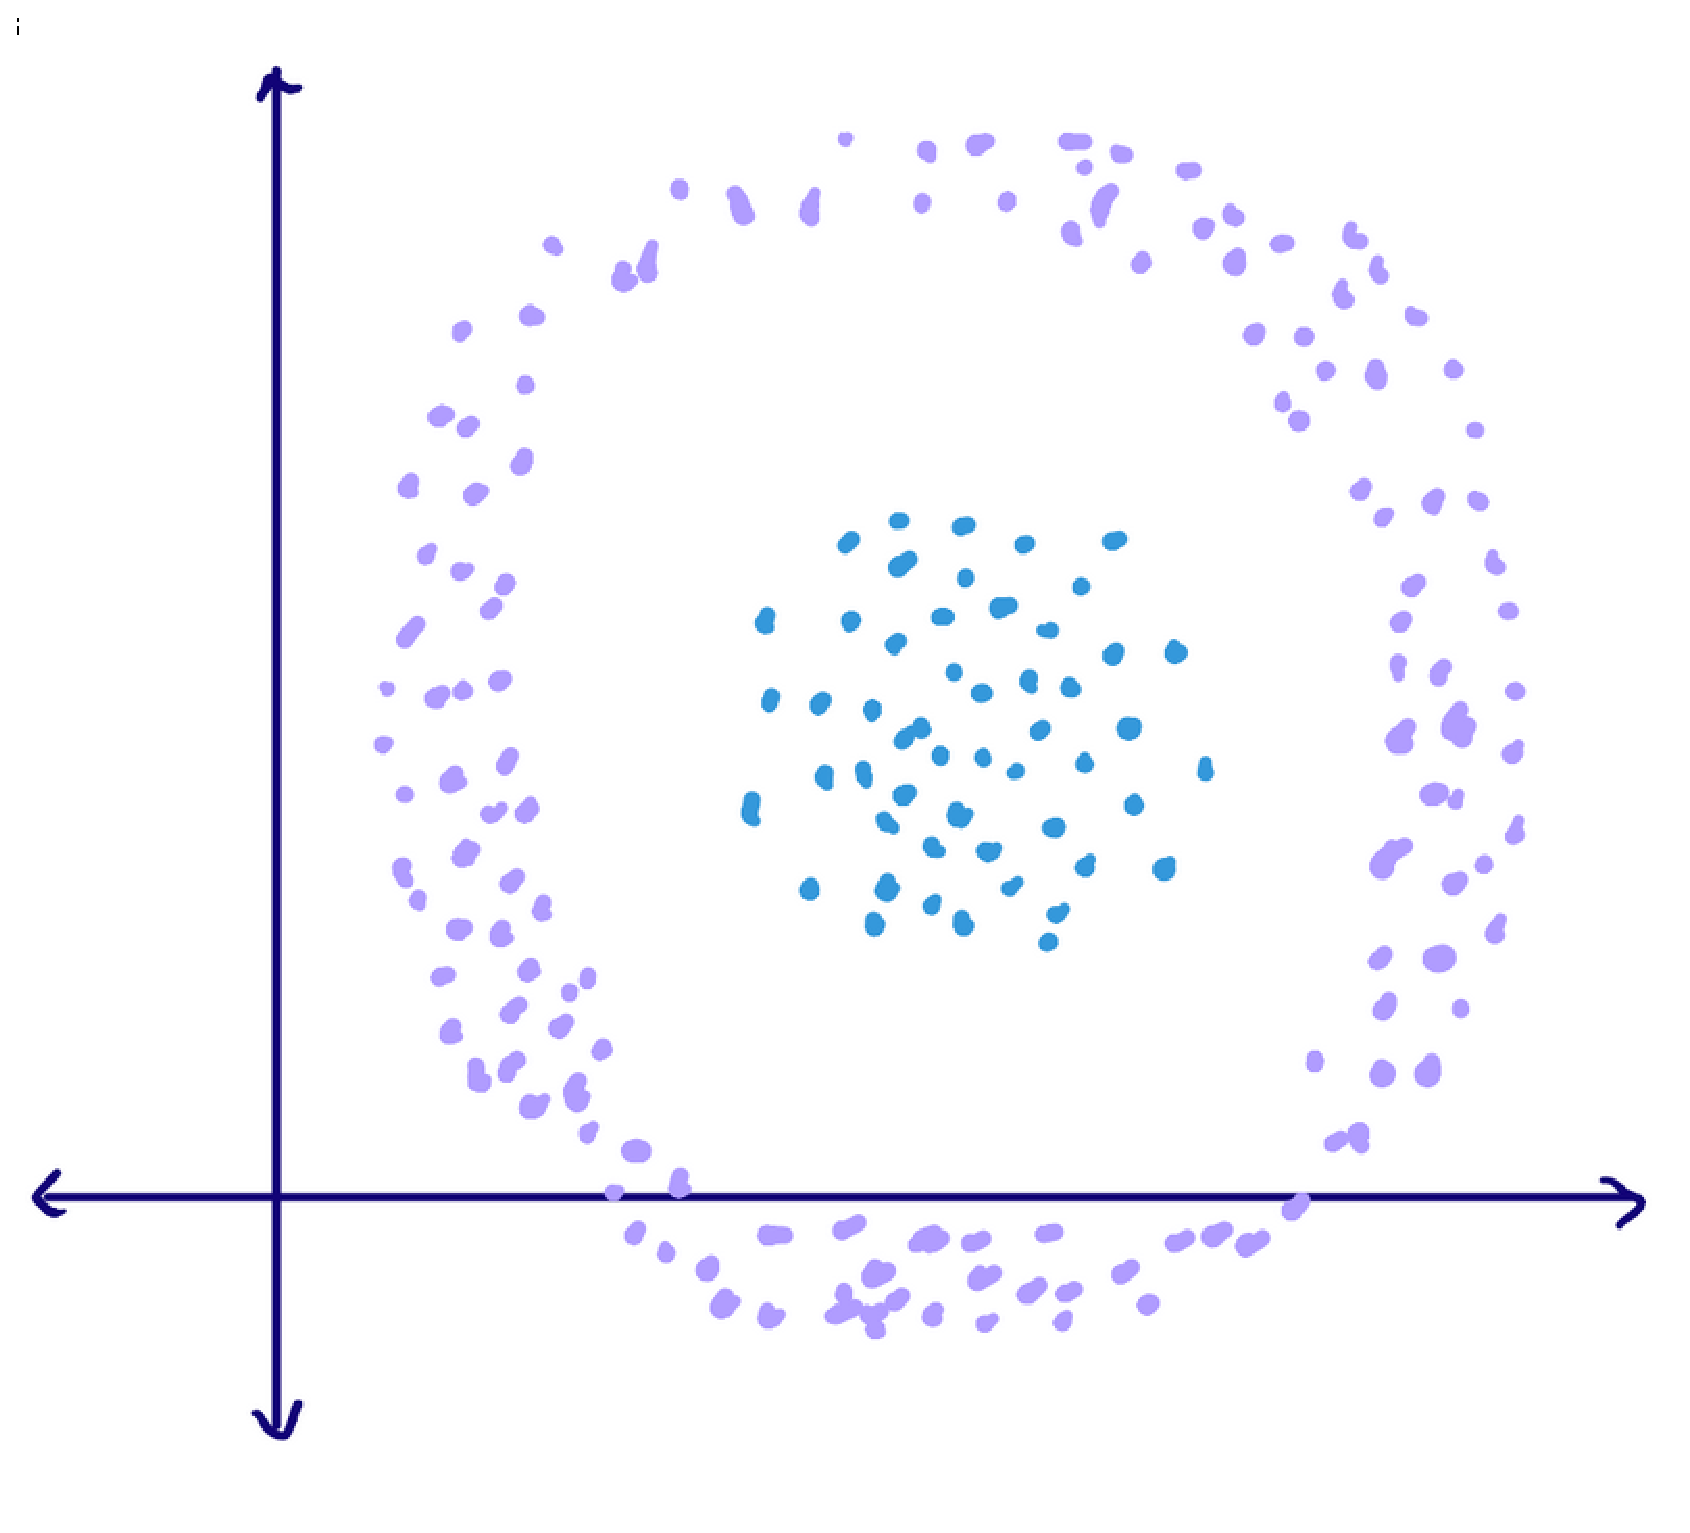
\includegraphics[width=3in]{../figures/arbitrary.eps}
    \end{center}
  \end{frame}

  \begin{frame}{Arbitrary Layer: What does it look like?}
    \begin{center}
      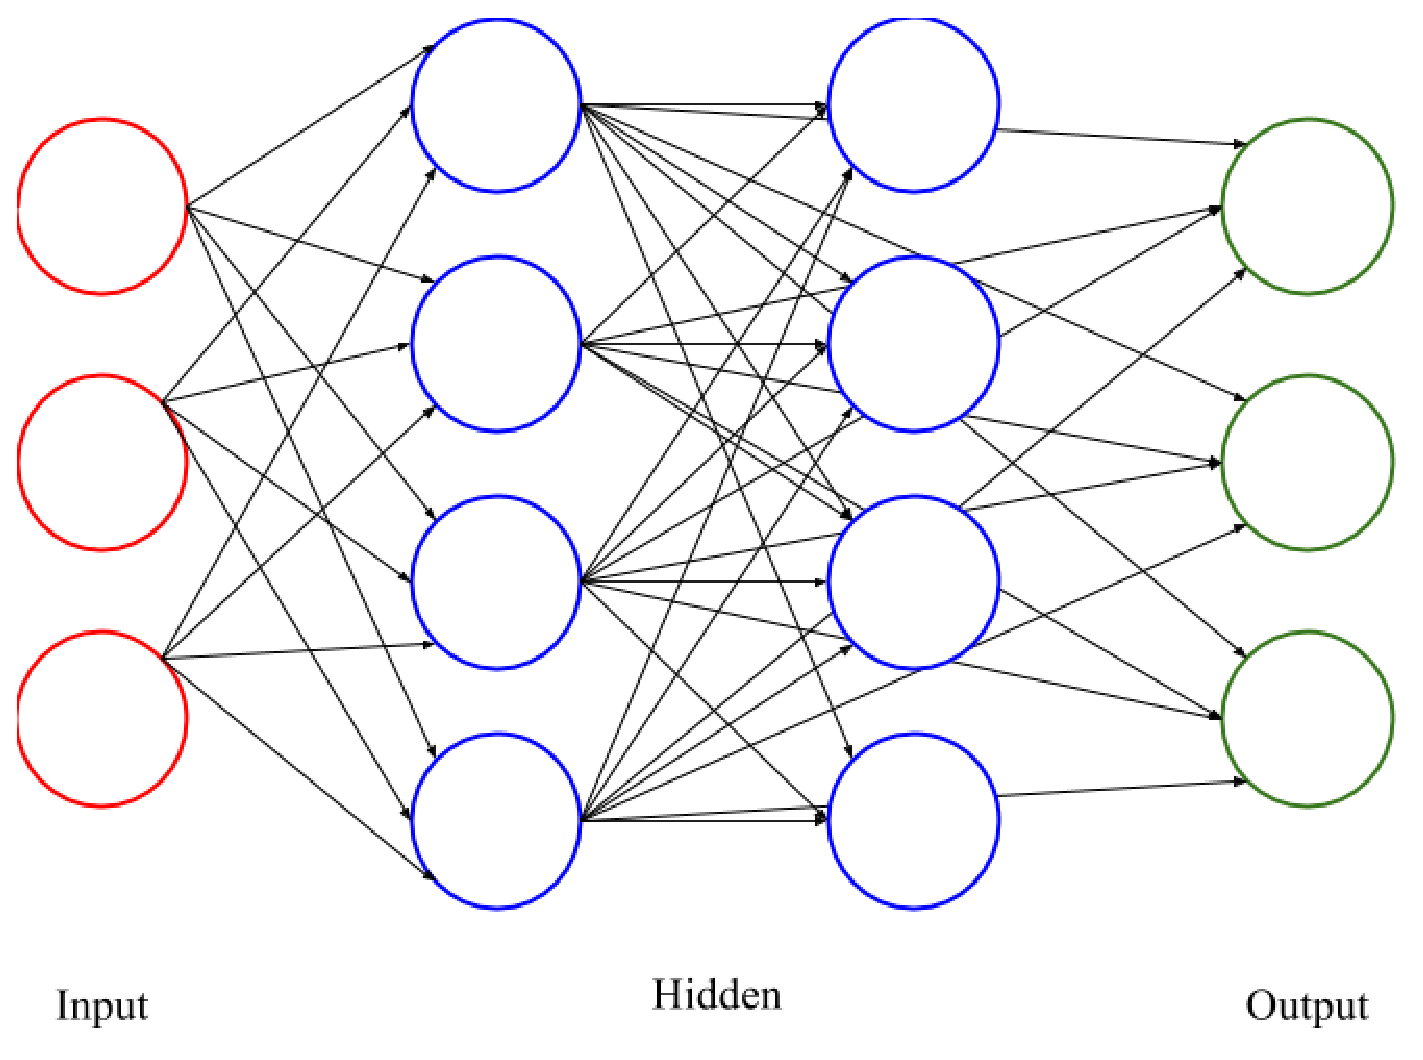
\includegraphics[width=3in]{../figures/deep_nn.eps}
    \end{center}
  \end{frame}

%  \begin{frame}{Arbitrary Layer NN}
%    As before:
%    \begin{enumerate}
%      \item forward propagation
%      \item backward propagation
%      \item update weights
%    \end{enumerate}
%  \end{frame}

  \begin{frame}{Arbitrary-Layer: Forward Propagation}
    For any layer $h$ in our network:
    \begin{itemize}
      \item parameters $W^{(h)}$ and $b^{(h)}$
      \item $A^{(h)} = Z^{(h-1)} W^{(h)} + b^{(h)}$
      \item $Z^{(h)} = \phi\left( A^{(h)} \right)$
    \end{itemize}

    Notes:
    \begin{itemize}
      \item $Z^{(0)} = X$ - aka training data is input for first layer
      \item output layer: just $P = Z^{(h)} W^{(h+1)} + b^{(h+1)}$
    \end{itemize}
  \end{frame}

  \begin{frame}{Arbitrary-Layer: Back Propagation}
    For each layer $h$, calculate $\nabla Z^{(h)}$ and pass to previous layer

    $$ \nabla A = \nabla Z_{out} \bullet 1\left( A > 0 \right).$$
    %$$ Z_{out}  = \phi\left( A \right). $$

    Just as for the single-layer network, we have
    $$ \nabla W = Z_{in} \nabla A, $$
    $$ \nabla b = \sum_{i=1}^m \nabla A_i. $$
    %$$ \nabla Z_{out} = \nabla AW. $$

    $$ \nabla Z_{in} = \nabla A W^T. $$

  \end{frame}

  \begin{frame}{Arbitrary-Layer: Update Weights}
    As before, we update our parameters with
      $$ W^{(h)} = W^{(h)} - \eta \nabla W^{(h)}, $$
      $$ b^{(h)} = b^{(h)} - \eta \nabla b^{(h)} $$
    for each layer $h$ in the network.
  \end{frame}

  \section{Implementation}

  \begin{frame}{Softmax Classifier, One-Layer Network}
    \begin{center}
      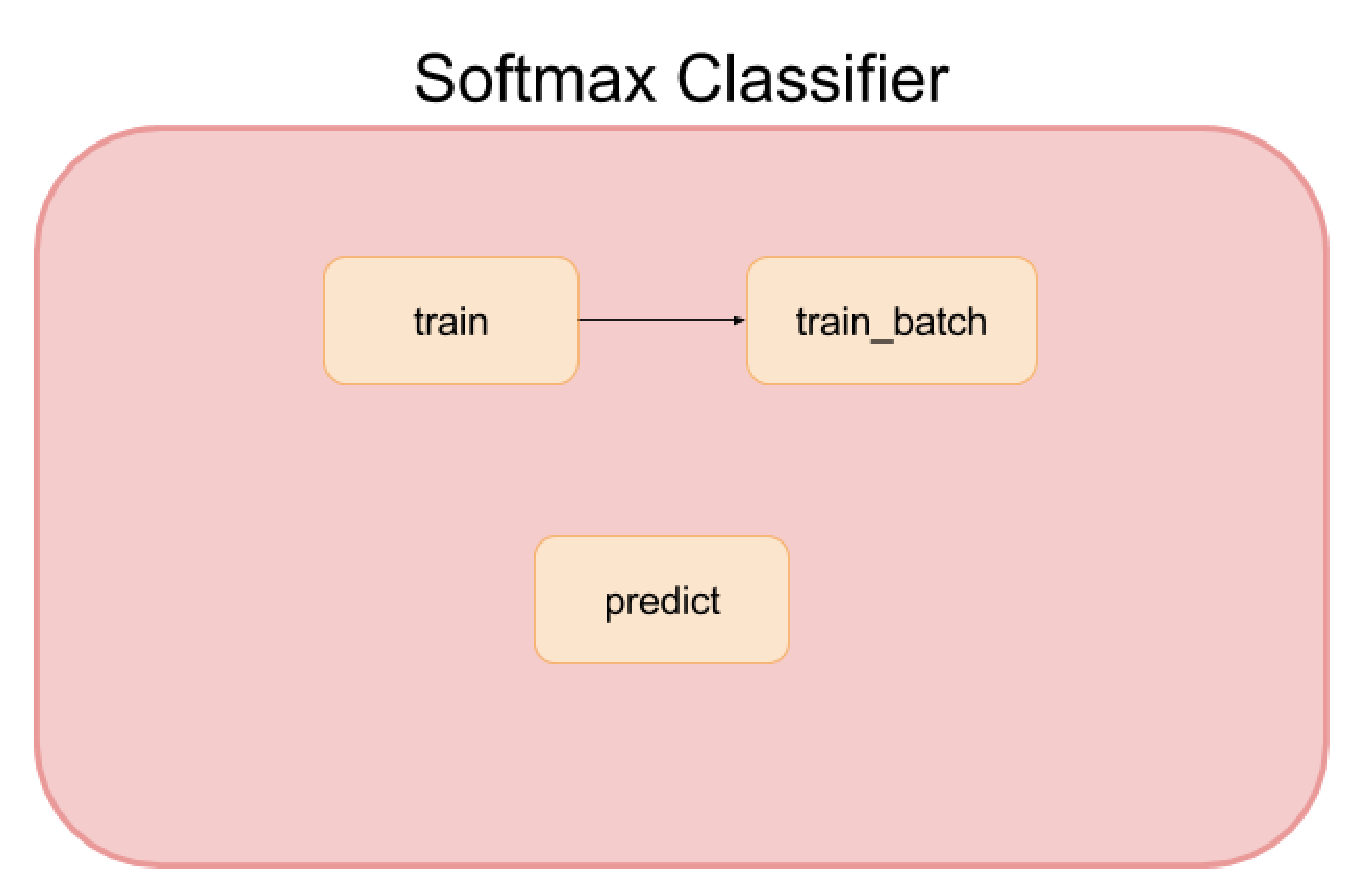
\includegraphics[width=3.5in]{../figures/softmax_drawing.eps}
    \end{center}
  \end{frame}

  \begin{frame}{Arbitrary-Layer Neural Network}
    \begin{center}
      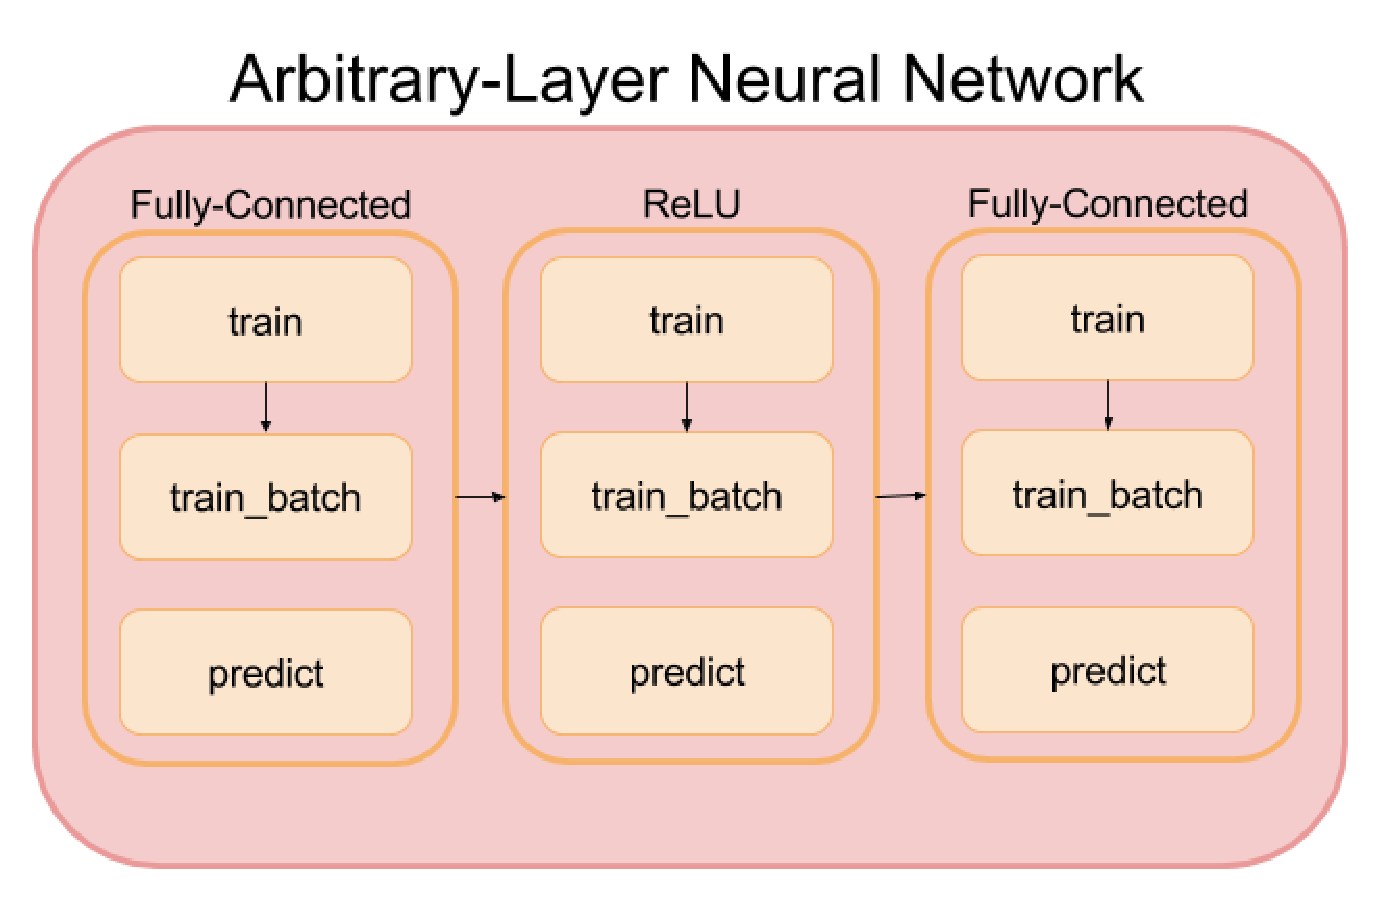
\includegraphics[width=3.5in]{../figures/arbitrary_drawing.eps}
    \end{center}
  \end{frame}

%  \begin{frame}[fragile]{Softmax Classifier}
%
%\begin{minted}{python}
%class SoftmaxClassifier:
%  def __init__(num_classes):
%    # initialize model parameters
%    ...
%  def train(X, y, batch_size, num_iterations, learning_rate):
%    # train classifier by calling train_batch
%    ...
%  def train_batch(X, y):
%    # performs forward pass, back prop, gradient update
%    ...
%  def predict(X):
%    # predict using best score for all images in X
%    ...
%\end{minted}
%
%{\ttfamily SingleLayer} object will have the same structure
%
%  \end{frame}
%
%  \begin{frame}[fragile]{Arbitrary Layer Neural Net}
%\begin{minted}{python}
%class NeuralNet:
%  def __init__(batch_size, epsilon, learning_rate, num_iters):
%    # initialize model parameters
%    ...
%  def add_layer(LayerType, input_size, output_size):
%    # add FullyConnected or Relu layer
%    ...
%  def train(X, y):
%    # calls forward and backward method on batches of X
%    ...
%  def forward():
%    # calls forward on each layer in network
%    ...
%  def backward():
%    # calls backward on each layer in network
%    ...
%  def predict():
%    # returns predictions using best score for all images in X
%    ...
%\end{minted}
%  \end{frame}
%
%  \begin{frame}[fragile]{Arbitrary Layer Neural Net}
%\begin{minted}{python}
%class FullyConnectedLayer:
%  def __init__(master, input_size, output_size, prev=None):
%    # master = NeuralNet object
%    # prev = previous layer, if not first layer
%    ...
%  def forward():
%    # preform forward pass on layer, pass to next layer
%    ...
%  def backward():
%    # perform back propagation on layer, pass to prev layer
%    ...
%  
%\end{minted}
%
%also have a {\ttfamily ReluLayer} class with the same methods
%  \end{frame}

  \section{Future Work}
  \begin{frame}{Future Work}
    Other Neural Network Architectures
    \begin{itemize}
      \item convolutional
      \item recurrent
    \end{itemize}
    Additional Neural Network features
    \begin{itemize}
      \item regularization
      \item batch normalization
    \end{itemize}
  \end{frame}

  \begin{frame}
    \begin{center}
      
\includegraphics[width=2.5in]{../figures/bitmoji.eps}
    \end{center}
  \end{frame}

  \section{Thank-you!}
\end{document}
